% ========== Chapter 1
 
\chapter {Neutrino Physics and \nonubb Introduction}
\section{Neutrinos as a Key to New Physics}
\subsection{The ``Desperate Remedy"}
Since its introduction by Wolfgang Pauli in 1930, the neutrino has been allowing physicists to reconcile theories and experimental results that did not quite align. At the time, the theories in question were the conservation of energy and angular momentum; beta decay observations seemed to violate these key principles. Instead of carrying away the full Q-value of the decay, the observed electrons could carry off a range of energies up to that value. And instead of exiting the interaction going back-to-back, as expected in a two-body decay under momentum conservation laws, the recoiling nucleus and electron could have any angle between them. 

As a ``desperate remedy," Pauli proposed the neutrino \cite{Pauli1930}-- a light, neutral particle that was being created in the decay, carrying off the missing energy and momentum. If it did not interact via the strong or electromagnetic forces, such a particle would be invisible to the beta decay experiments. In fact, the elusive neutrino escaped detection for over twenty years, until it was eventually observed in 1956 \cite{Cowan1956}. With the addition of this particle to the standard model, beta decay was explained as a three-body process, and the conservation laws were saved.

\subsection{The Solar Neutrino Problem}
Along with the neutrino, the concepts of lepton number and lepton number conservation were introduced. This value, in the standard model, is conserved in weak interactions, which proceed via two classes of vertex, called the neutral and charged currents. The Feynman diagrams for these processes are seen in Fig.~\ref{weak_diagrams}. In the charged current interactions, a charged lepton (i.e. the electron, muon, or tau, or their antiparticles) participates in the interaction, and the (anti-)neutrino always occurs with the W+(-) boson. In the neutral current interaction, a lepton and its corresponding anti-lepton occur along with the Z boson. 

\begin{figure}[h]
\hfil 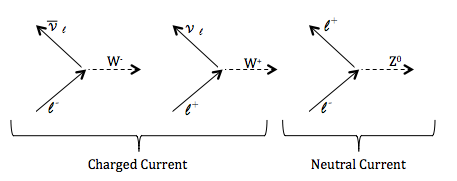
\includegraphics[width = .80\textwidth]{/Users/jgruszko/Documents/Thesis/Images/Ch1/WeakDiagrams.png} \hfil
\caption[Feynman diagrams for the weak interactions]{The primitive vertices of the Feynman diagrams for weak interactions between leptons in the standard model. Equivalent vertices exist for the quarks. \cite{PDG2014}}
\label{weak_diagrams}
\end{figure}

There are three observed active neutrino flavors, corresponding to the three charged leptons, which form a basis of flavor eigenstates. They are created in these eigenstates; in a charged current interaction emitting an electron, for instance, the standard model requires that an electron anti-neutrino is also created. Originally, it was believed that neutrinos also followed lepton-flavor conservation. Since in the standard model, neutrinos are massless, that electron anti-neutrino would propagate in its flavor eigenstate, and remain an electron anti-neutrino. 

With this assumption firmly in place, physicists attempted to detect the neutrinos created in the sun. Ray Davis and his team, in the Homestake experiment (housed in the predecessor to today's Sanford Underground Research Facility), used a radiochemical technique based on the inverse beta decay $\nu_{e} + ^{37}Cl \rightarrow ^{37}Ar + e^-$ to measure the integrated flux of $\nu_e$ with energies over 0.518\,MeV. Based on astrophysical models of solar fusion processes, over 6 SNU (Solar Neutrino Units, a unit equivalent to one interaction per $10^{36}$ target atoms per second) were expected \cite{TurckChieze1993} \cite{Bahcall1995}. Measurements from Davis's and other solar neutrino experiments, however, consistently found about a third the flux that these models predicted \cite{Davis1998}. Once again the theory and the experimental results did not agree.

As in the 1930s, the unexpected physics of the neutrino saved the day. If the neutrino was not massless, as the Standard Model seemed to assert, but instead had a small mass, it would not propagate in its flavor eigenstate. Instead it would propagate in a mass eigenstate, and if these eigenstates were not equivalent, it would change from one flavor to another as it traveled from the sun to detectors on earth. Experiments like Davis's, which were sensitive only to electron-type neutrinos, would see fewer events than expected, but the deficit would appear as a surplus in the muon- and tau-type neutrino fluxes. 

Testing this theory required detectors that could measure the total neutrino flux, instead of just the flux of $\nu_e$. With the construction of the Super-Kamiokande and SNO experiments, the total neutrino flux could finally be measured. By 2001, the existence of neutrino oscillations had been confirmed \cite{SuperK1998} \cite{SNO2001}, and the solar models rescued. 

\subsection{Measuring Neutrino Properties}
The mixing of the mass eigenstates in a given flavor eigenstate is described by the unitary Pontecorvo-Maki-Nakagawa-Sakata (PMNS) matrix, 
\begin{equation}
\begin{bmatrix}
\nu_e\\
\nu_\mu\\
\nu_\tau\\
\end{bmatrix}
=
\begin{bmatrix}
U_{e1} & U_{e2} & U_{e3} \\ 
U_{\mu1} & U_{\mu2} & U_{\mu3} \\ 
U_{\tau1} & U_{\mu2} & U_{\mu3} \\ 
\end{bmatrix}
\begin{bmatrix}
\nu_1\\
\nu_2\\
\nu_3\\
\end{bmatrix}
\label{eqn:PMNS}
\end{equation}
where $\nu_1$, $\nu_2$, and $\nu_3$ are the three distinct neutrino mass eigenstates and the $U_{ij}$ are the mixing parameters. The matrix is generally parameterized using three mixing angles $\theta_{12}, \theta_{23}, \theta_{13}$ and a single phase $\delta_{CP}$ that describes the quantity of charge-parity symmetry violation. In that case, the PMNS matrix can be expressed as:
\begin{equation}
U = 
\begin{bmatrix}
1 & 0 & 0 \\ 
0 & \cos\theta_{23} &\sin\theta_{23} \\ 
0 & -\sin\theta_{23} & \cos\theta_{23} \\ 
\end{bmatrix}
\begin{bmatrix}
\cos\theta_{13}  & 0 & \sin\theta_{23}e^{-i\delta_{CP}} \\ 
0 & 1 & 0 \\ 
0 & -\sin\theta_{23}e^{-i\delta_{CP}} & \cos\theta_{13} \\ 
\end{bmatrix}
\begin{bmatrix}
\cos\theta_{12}  & \sin\theta_{12} & 0  \\ 
-\sin\theta_{12} & \cos\theta_{12} & 0 \\ 
0 & 0 & 0 \\ 
\end{bmatrix}
\hspace{-10pt}
\label{eqn:PMNS_angle}
\end{equation}
This is the parametrization generally used to describe the results of neutrino oscillation experiments. In general, the neutrino oscillation angles $\theta_{ij}$ have been observed to be large, unlike the equivalent mixing angles in the quark sector \cite{PDG2014}. 

The probability of neutrino oscillation from one flavor, $\alpha$, to another, $\beta$, is:
$$ 
P_{\alpha\beta} = \left|\sum_i U^*_{\alpha i} U_{\beta i} e^{-im_i^2 L/2E}\right|^2
$$
where $L$ is the baseline length of the oscillations (i.e., the distance traveled by the neutrino), $E$ is the energy of the neutrino, $m_i$ is the mass of the each mass eigenstate, and the $U_{\alpha(\beta) i}$ are as in Eqn.~\ref{eqn:PMNS} and~\ref{eqn:PMNS_angle}. 

To see the the salient features of the mixing, we can instead examine the simplified case of two-flavor mixing:
$$ 
P_{\alpha\beta} = \sin^2(2\theta)sin^2\left(\frac{\Delta m^2 L}{4E}\right)
$$
where $\theta$ is the mixing angle between the two mass eigenstates, and $\Delta m^2 \equiv m_1^2-m_2^2$. As seen here, the mixing between the flavors depends only on the mass-squared difference between the states, and not on the state masses themselves, or on the sign of the differences between the masses. 

The same holds true in the full 3-flavor case. Therefore, in spite of the fact that the mixing parameters and mass-splittings (the $\Delta m_{ij}$) have been measured to fairly high accuracy by oscillation experiments, we still have limited information about the other neutrino properties. 

The sign of $\Delta m_{ij}^2$ does appear in the oscillation probability when the neutrino passes through matter, instead of through vacuum, during its travel. The amount of matter needed for the sign determination at current oscillation measurements' sensitivity levels is large. At the moment, only the sign of $\Delta m_{12}^2$, also called $\Delta m_{sol}^2$, is known. In this case, the neutrino's travel through the sun can be leveraged. From solar neutrino oscillation experiments like SNO, SuperK, and KaMLAND it is known that $m_2 > m_1$ \cite{PDG2014}. 

Several experiments plan to determine the sign of $\Delta m_{23}^2$, also called $\Delta m_{atm}^2$, in the coming decade \cite{Cahn2013}, some by detecting laboratory-produced beams of neutrinos at long baselines, like DUNE, and others by measuring the effect of the earth's matter on atmospheric neutrinos, like PINGU and HyperK.  At the moment, however, the sign of $\Delta m_{23}^2$ is unknown, leading to what are called the ``normal" and ``inverted" possible cases of the neutrino mass hierarchy, as seen in Fig.~\ref{mass_hierarchy}  \cite{Hewett2012}. 

The normal hierarchy (NH) is referred to as such by analogy to the masses of the charged leptons, since the small splitting between the two lightest species mimics the similar masses of the $e$ and $\mu$, with the $\tau$ being significantly heavier. However, both hierarchies are considered to be equally natural under the SM. 

\begin{figure}[]
\hfil 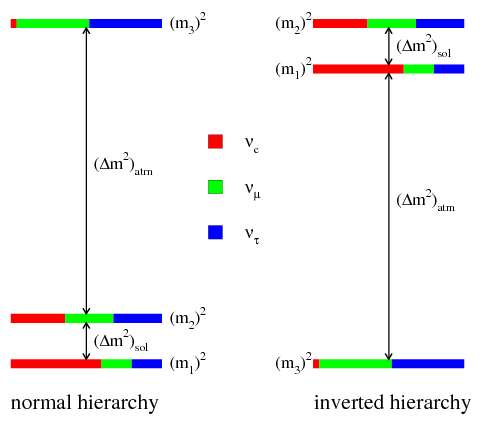
\includegraphics[width = .40\textwidth]{/Users/jgruszko/Documents/Thesis/Images/Ch1/MassHierarchy.png} \hfil
\caption[The two possibilities for the neutrino mass hierarchy]{The two possible cases of the neutrino mass hierarchy \cite{Hewett2012}. The sign of $\Delta m_{12}^2$ is known, but the sign of $\Delta m_{23}^2$ (or, equivalently, $\Delta m_{23}^2$) is not known.}
\label{mass_hierarchy}
\end{figure}

The overall mass of each of the eigenstates is also unknown. Direct mass measurements studying the shape of $\beta$ decay spectra are sensitive to the mix of mass eigenstates of the electron-flavor neutrino: 
$$m(\nu_e)^2 = \sum_i \left|U^2_{ei}m(\nu_i)\right|^2 $$
The most sensitive such limits come from the Mainz \cite{Mainz2005} and Troitsk \cite{Troitsk2011} measurements of tritium ($^3$He) decay, which have set upper limits of 2.3 and 2.05\,eV, respectively, on $m(\nu_e)$. 

More stringent limits, below 0.23\,eV, have been derived from cosmic microwave background observations \cite{PlanckXVI_2013}, which are sensitive to the sum of the neutrino masses $\sum m_i$. These measurements, however, are highly model-dependent. The KATRIN experiment plans to directly probe masses down to $m(\nu_e) \sim 0.20$\,eV \cite{KATRIN2015}. 

The CP symmetry-violation phase $\delta_{CP}$ is also unknown. This parameter drives the potential difference between the oscillation of the left-handed active neutrinos, and the right-handed active antineutrinos. If charge parity (CP) symmetry is conserved, their oscillation probabilities will be identical; any deviation indicates $\delta_{CP} \neq 0$. Current measurements from neutrino beam experiments like NO$\nu$A weakly disfavor CP conservation \cite{NOvA2016}. 

\subsection{The Origins of Neutrino Mass}
Because neutrino oscillations have been observed, at least two of the neutrino mass eigenstates are required to be non-zero. The Standard Model description of how particles get their mass, however, cannot be straightforwardly applied to the neutrino. 

\subsubsection{The Dirac Mass Mechanism}
In the SM, fermions are described by a combination of four independent fields. Electrons, for instance, are described with the fields ($e_L$, $\overline{e_L}$, $e_R$, $\overline{e_R}$), where $L$ and $R$ refer to left- and right-chiral fields and the bar refers to charge-conjugation, i.e., the positron $e^+$. Such Dirac particles receive their masses through interaction with the Higgs field, which couples the left- and right-chiral fields of the same charge to one another. In other words, the Higgs interaction changes the particle's parity, but not its charge. 

In the SM, however, the right-chiral neutrino field $\nu_R$ and the left-chiral antineutrino field $\overline{\nu_L}$ do not exist; since the weak-interaction is maximally parity-violating, such fields would be sterile. In other words, the W$^{+(-)}$ and Z bosons would not couple to them, and they would be non-interacting. Unlike in the charged particles of the SM, they are not needed to fully describe the interactions we observe.

These fields can be added to the SM, making the neutrino a Dirac particle and granting it mass via the Higgs mechanism. This mass mechanism, however, leaves a fine-tuning problem. Current limits indicate that the neutrino mass is five to six orders of magnitude smaller than the masses of the other standard model particles, and the theory provides no justification for this large difference. 

\subsubsection{The Majorana Mass Mechanism}
Since the neutrino is neutral, the four independent Dirac fields are not needed to fully describe it. Instead, the neutrino could be described by just two fields, $\nu_L$ and $\nu_R$. The left-chiral field, in this case, corresponds to the particle we observe as the neutrino, and the right-chiral field to the one we observe as the antineutrino. This would make the neutrino a Majorana particle.

In this case, the particle would receive its mass from the Majorana mass mechanism, which changes the particle's parity and its charge. The left-handed mass term, which couples $\overline{\nu_R}$ to $\nu_L$, is required to exist by our observations. On its own, however, it is not renormalizible; some sort of Beyond-the-Standard-Model physics is needed, whether the right-handed Majorana mass term (and therefore the sterile neutrino fields $\nu_R$ and $\overline{\nu_L}$) or some other massive particle.  

The Majorana mass mechanism violates lepton-number conservation and allows for the possibility of additional CP-violation. The PMNS matrix, parametrized as in Eqn.~\ref{eqn:PMNS_angle}, receives an additional term with up to two Majorana CP-violation phases $\alpha_1$ and $\alpha_2$:
$$
U^\prime = U 
\begin{bmatrix}
1 & 0 & 0 \\ 
0& e^{i\frac{\alpha_{1}}{2}} & 0 \\ 
0& 0 & e^{i\frac{\alpha_{2}}{2}} \\ 
\end{bmatrix}
$$

Since the mass mechanism is completely different than that of the other SM particles, there is no unnaturalness argument to overcome in this case. In fact, the Majorana mass mechanism can be used to explain the smallness of the neutrino mechanisms, through what is known as the ``see-saw mechanism."

\subsubsection{The See-Saw Mechanism and Other Remedies}
An intriguing possibility for the origin of the neutrino mass is the see-saw mechanism, in which the neutrino has both Dirac and (left- and right-handed) Majorana masses. In this case, the 4 degenerate-mass Dirac fields of the neutrino are split into two lighter and two heavier fields by the addition of the Majorana mass term. 

When both of these terms are included, the Lagrangian for the neutrino mass becomes:
$$ L_{mass} = 
\frac{1}{2} \left(\overline{\nu_L}~\overline{\nu_R}^c\right) \
\begin{bmatrix}
M_L & m_D  \\ 
m_D & M_R  \\ 
\end{bmatrix}
\begin{bmatrix}
\nu_L^c  \\ 
\nu_R   \\ 
\end{bmatrix}
+ h.c.
$$
where $M_L$ and $M_R$ are the left- and right-handed Majorana mass terms, $m_D$ is the Dirac mass term, and $h.c.$ indicates the Hermitian conjugate of the first term.

If $M_L\rightarrow 0$, diagonalizing this matrix leaves two particles:
$$ L_{mass} = 
 \left(\overline{\nu}~\overline{N}\right) \
\begin{bmatrix}
\frac{m_D^2}{M_R} & 0  \\ 
0 & M_R  \\ 
\end{bmatrix}
\begin{bmatrix}
\nu  \\ 
N   \\ 
\end{bmatrix}
$$
where we have identified the particle with the correct handedness (i.e. a left-handed particle and a right-handed antiparticle) as the neutrino $\nu$, and the new particle as $N$. 

The $\nu$ then has mass $\frac{m_D^2}{M_R}$, and the new opposite-handed particle $N$ has mass ${M_R}$. If $m_D$ is about 100\,GeV, similar to the other Dirac masses, and $m_R$ is of the same order as the GUT scale, about 10$^{15}$\,GeV, then the neutrino mass would be about 10\,meV, similar to the neutrino mass implied by current limits. The new particle $N$ would be a heavy right-handed neutrino that is only present in the early universe. 

Thus, the see-saw mechanism provides a natural explanation for the smallness of the observed neutrino mass. The Majorana mass mechanism also allows leptogenesis, which in combination with the new heavy right-handed neutrino $N$ could provide a mechanism for baryogenesis in the early universe, explaining the matter/anti-matter imbalance in the observable universe \cite{DiBari2012}. The unexpected physics of the neutrino could once again provide a remedy to some of the problems of our current understanding of fundamental physics. 
	
\section{Neutrinoless Double Beta Decay}
\subsection{\nonubb Theory}
The most promising process by which to discover the nature of the neutrino is neutrinoless double beta decay. 

In standard-model two neutrino double-beta decay, a nucleus that contains an even number of nucleons is energetically forbidden from decaying via single beta-decay. Instead, two beta decays occur, leading to the emission of two electrons and two electron anti-neutrinos:
$$X(A, Z) \rightarrow X(A, Z+2) + 2 e^{-} + 2 ~\overline{\nu_e}$$
as shown in Fig.~\ref{fig:2nBB}. This second-order process has a very long half-life  ($t_1/2 > 10^{18}$\,yrs), but is predicted under the Standard Model and has been observed in a dozen different nuclei \cite{Barabash2010}. 

If the neutrino is Majorana, an even rarer process could occur: instead of emitting two antineutrinos, the antineutrino could be exchanged within the nucleus as a virtual particle. In other words, it functions as an outgoing antineutrino for one of the $\beta$ decays, and as an incoming neutrino for the other decay, as shown in Fig.~\ref{fig:0nBB}. Thus, no neutrinos are seen in the final state:
$$X(A, Z) \rightarrow X(A, Z+2) + 2 e^{-},$$
and all of the energy of the decay is carried by the electrons. Due to momentum conservation, the nucleons carry a negligible amount of the energy. 

 \begin{figure}[h]
 \centering
    \begin{subfigure}[t]{.40\textwidth}
      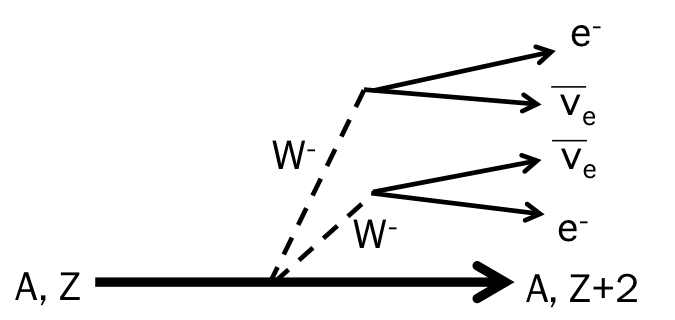
\includegraphics[width =\textwidth]{/Users/jgruszko/Documents/Thesis/Images/Ch1/2nBB.png}
       \caption{Standard Model-allowed \twonubb.}
        \label{2nBB}
        \end{subfigure}   
         \hfil
        \begin{subfigure}[t]{0.4\textwidth}
      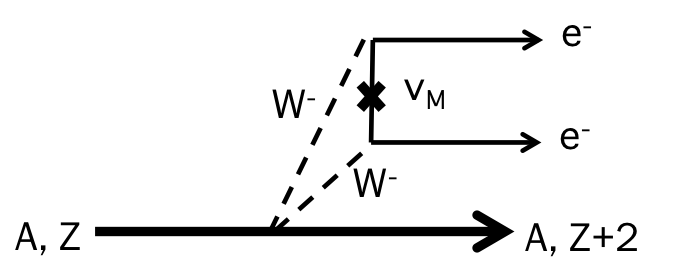
\includegraphics[width =\textwidth]{/Users/jgruszko/Documents/Thesis/Images/Ch1/0nBB.png} 
      \caption{\nonubb, which can only occur if the neutrino is Majorana. The cross indicates the appearance of a Majorana mass term.}
      \label{0nBB}
    \end{subfigure}   
    \caption{Feynman diagrams for double-beta decay processes.}
\end{figure}

This decay relies on the non-conservation of lepton number, on the Majorana nature of the neutrino, and on the fact that the emitted neutrino is in a mixed helicity state. Because of the last consideration, the effective size of the Majorana mass term, 
 $$\langle m_{\beta\beta} \rangle = |\sum\limits_{i=1}^3 U^2_{ei}m_i|,$$
 where $U_{ei}$ is the mixture of neutrino mass eigenstates $i$ in the electron neutrino, appears in the $0\nu\beta\beta$ rate:
 \begin{equation}
 (T_{1/2}^{0\nu})^{-1} = G^{0\nu}|M_{0\nu}|^{2}\left(\frac{\langle m_{\beta\beta} \rangle}{m_e}\right)^2 .
 \label{eqn:0nBBrate}
 \end{equation}
 $G^{0\nu}$ is a phase space factor, $M_{0\nu}$ is the nuclear matrix element, and $m_e$ is the electron mass. 

The half-life in Eqn.~\ref{eqn:0nBBrate} only holds for double-beta decay via the exchange of a light Majorana neutrino, the minimal model by which it can occur. However, this observed decay could also occur via a variety of other, more exotic mechanisms, all of which would imply that the neutrino is a Majorana particle and that lepton number is not conserved \cite{Schechter1982}. 
 
Because they contribute to $m_{\beta\beta}$, both the overall neutrino mass and the mass hierarchy can contribute to the observed rate, as seen in Fig.~\ref{0nBBrate}. Here we see that if the neutrino masses are large compared to the size of the mass splittings, the mass hierarchy does not significantly affect $m_{\beta\beta}$. If, on the other hand, the neutrino masses are similar in scale to the mass splittings, having two heavier neutrinos and only one lighter neutrino, as in the IH, leads to a higher $m_{\beta\beta}$ and a higher \nonubb\ rate than the NH at an equivalent lightest neutrino mass. 
 
Additionally, in the NH, unlike in the IH, the two Majorana phases $\alpha_1$ and $\alpha_2$ can lead to complete cancellation of $m_{\beta\beta}$ at certain neutrino masses, seen in Fig.~\ref{0nBBrate} as the region in which the allowed $m_{\beta\beta}$ band extends to 0. In Bayesian models of the discovery potential of future \nonubb\ experiments, the probability of such a combination of parameters depends strongly on the prior used to model the neutrino masses. It has been discussed extensively in recent analyses \cite{Agostini2017} \cite{Caldwell2017}. 
 
  \begin{figure}[h]
 \centering
 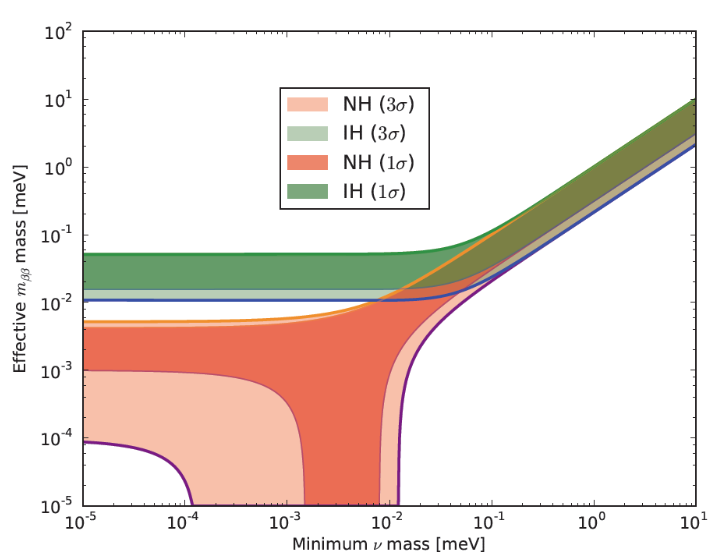
\includegraphics[height=3in]{/Users/jgruszko/Documents/Thesis/Plots/Ch1/0nBB_Rate.png}
  \caption[$m_{\beta\beta}$ dependence on the neutrino mass and hierarchy]{$m_{\beta\beta}$, and therefore the $0\nu\beta\beta$ rate, depend on the neutrino mass hierarchy and the overall mass scale \cite{ZuberINT2015} .}
  \label{0nBBrate}
  \end{figure}   
  
The well-understood behavior of $m_{\beta\beta}$, and therefore $(T_{1/2}^{0\nu})^{-1}$, makes \nonubb\ an exciting prospect for experimental study. One hopes to detect \nonubb, of course, but even a null signal provides information about the nature of the neutrino, particularly when combined with other experiments that could determine the neutrino mass and mass hierarchy. 

Conversely, a measurement of $(T_{1/2}^{0\nu})^{-1}$ would provide information about the neutrino mass and possibly determine the neutrino mass hierarchy. There would be some uncertainty in these determinations, since experimental results must be translated from a measurement of $(T_{1/2}^{0\nu})^{-1}$ to a value of $m_{\beta\beta}$, which involves the uncertain matrix element for the nucleus in question. If \nonubb\ were detected in multiple isotopes, however, the effects of this uncertainty would be mitigated. 

Most reassuringly, the search for \nonubb\ (at least, via light Majorana neutrino exchange) has a natural stopping-point; the rate of the decay, at almost all neutrino masses, cannot be infinitely long. 

\subsection{Observing 0$\nu\beta\beta$}
Since no energy is carried away by neutrinos, the entire energy difference $Q$ between the initial- and final-state nucleus undergoing double-beta decay is carried by the outgoing electrons. Since double-beta decay experiments measure the sum of the electron energies, the experimental signature of such a decay would be a delta peak in energy at the endpoint of the two-neutrino mode spectrum, as in Fig.~\ref{0nBBspectrum}.

\begin{figure}[]
\centering
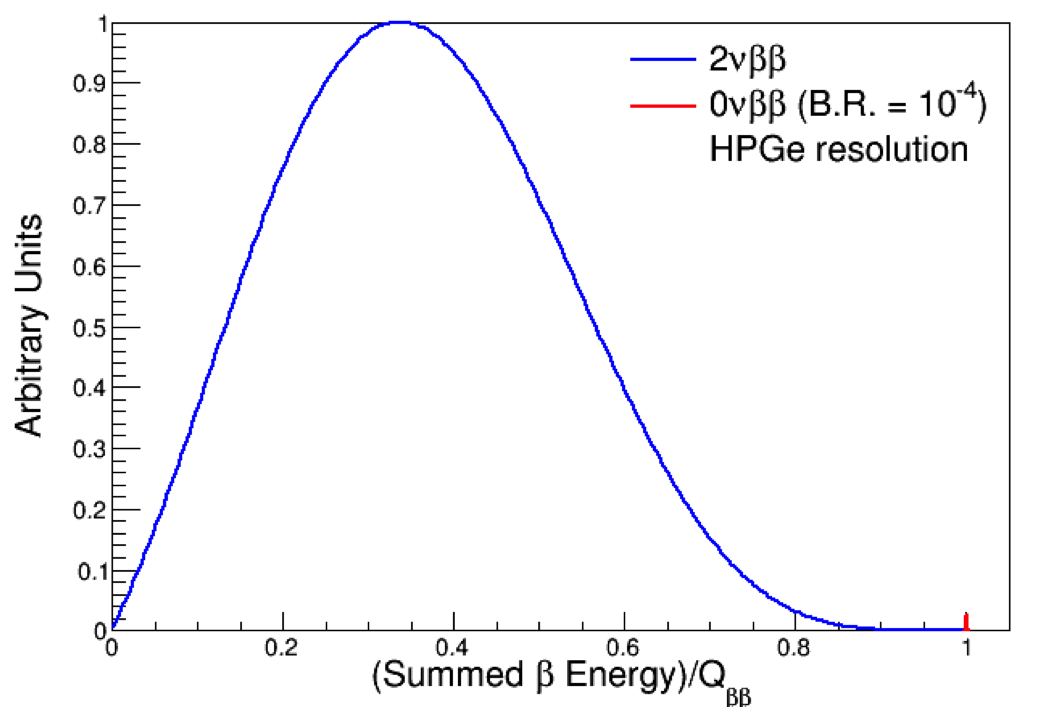
\includegraphics[height=3in]{/Users/jgruszko/Documents/Thesis/Plots/Ch1/DoubleBetaEnergy.png} 
      \caption[The experimental signature of $0\nu\beta\beta$ decay as it would appear in \iso{76}{Ge}]{The experimental signature of $0\nu\beta\beta$ decay as it would appear in \iso{76}{Ge}. Plot courtesy of Jason Detwiler.}
      \label{0nBBspectrum}  
\end{figure}

The challenge in detecting \nonubb\ comes from its extremely low rate. Current limits set the $0\nu\beta\beta$ half-life to greater than $10^{25}$ years \cite{EXO2014}. To observe such a rare decay, backgrounds of $0\nu\beta\beta$ experiments must be extremely low, and the mass of source material must be as large as possible. 

Several strategies are commonly used by the $0\nu\beta\beta$ community. Some are determined solely by the choice of source material:
\begin{itemize}
\item Q Value: The higher the Q-value of the $0\nu\beta\beta$ decay in some material, the less background contamination will occur in the signal region. While incomplete energy collection, Compton scattering, and other processes can cause background events to appear at energies below the peak value of the decay, events generally cannot gain energy by any process. 
\item Enrichment: Source materials often have to be enriched in the $0\nu\beta\beta$ isotope to allow for higher source masses without increasing backgrounds. The ease and expense of this process varies widely depending on the material, as does the need for enrichment.
\item Favorable Matrix Elements: $M_{0\nu}$ varies between isotopes; a favorable rate could increase the $0\nu\beta\beta$ rate. However, different calculation strategies lead to variation in these values that is on the order of the difference between isotopes. See \cite{Simkovic2009} for further discussion. 
\item Low $2\nu\beta\beta$ Rate: The resolution of any detector is imperfect, so events from the high-energy tail of the $2\nu\beta\beta$ will contribute to the background. The $2\nu$ rate is unrelated to the $0\nu$ rate, so a lower \twonubb\ rate reduces backgrounds without affecting the \nonubb\ rate.
\end{itemize} 
Unfortunately, there is no ``magic bullet" isotope for $0\nu\beta\beta$ that has all the favorable properties. 

Other strategies for background reduction are affected by the detector technology used and the design of the experiment:
\begin{itemize}
\item Source as Detector: Using the same material for both source and detector increases efficiency and makes it easier to increase source mass without increasing backgrounds.
\item Surface Event Rejection and Fiducial Volume Cuts: Generally, the bulk of the source/detector material is low in background, and most background events are from surface contamination, external sources or other components of the experiment. Detection strategies that allow surface events to be removed from the data set can often reduce backgrounds by taking advantage of self-shielding.
\item Multi-Site Rejection and Particle Identification: Many backgrounds are from $\gamma$ and $\alpha$ particles. The former often lead to multi-site interactions, while $0\nu\beta\beta$ is by its nature a single-site process, since electrons have much a shorter mean-free-path than photons in detector materials. If the detector can distinguish between multi-site and single-site interactions, backgrounds can be reduced. $\alpha$ backgrounds can be distinguished from $e/\gamma$ interactions in many two-energy-channel detectors, like time projection chambers and scintillating bolometers, and similarly reduced. 
\item High Resolution: Higher resolution makes background events easier to identify and shrinks the region of interest (ROI) for $0\nu\beta\beta$ decay, making background requirements less stringent.
\item Low Thresholds: Low energy thresholds are not required, but can allow better identification of high-energy backgrounds through timing cuts that search for L- and K-shell decay peaks of short-lived intermediate states of certain background decays. 
\item Large Overburden: All competitive $0\nu\beta\beta$ decay experiments are housed underground, to decrease the rate of cosmic-ray backgrounds and cosmogenic activation of detector materials. 
\end{itemize}
This work focuses on improving an existing \nonubb\ experiment via the development of pulse-shape based identification of surface $\alpha$ events, a strategy that falls under two of these bullet points. 

\subsection{Backgrounds and 0$\nu\beta\beta$ Sensitivity}


\subsection{\nonubb\ Searches in $^{76}$Ge}
$^{76}$Ge has several advantages as a choice of isotope for \nonubb\ searches, both in its innate properties and when used to create semiconductor diode detectors. 

Its Q-value, at 2.039\,MeV, is above the energies of most gamma background events. The only potentially significant environmental gamma background contributions are from $^{208}$Th and $^{214}$Bi decay in the $^{232}$Th and $^{238}$U chains, respectively. Other potential gamma background contributions come from cosmogenic activation of the detector and other materials in the experiment, in the form of $^{68}$Ge and the sum-peak of $^{60}$Co decay. Finally, muon-induced neutron spallation in the materials surrounding the detector could also lead to high-energy high energy gamma cascades, though these events are rare for experiments with large overburdens.

Natural-abundance Ge, which is 7.75\% $^{76}$Ge, can be enriched to over 87\% $^{76}$Ge. Though this process is expensive, it is well-understood, and both the facilities and raw material exist to enrich the large quantities needed for current and future experiments. 

The biggest advantages of  $^{76}$Ge \nonubb\ searches come from the detector technologies that can be used with this isotope. High-Purity Ge (HPGe) detectors are intrinsically very pure, giving them low internal backgrounds. They have a long history in nuclear physics and rare-event searches, so the techniques needed to operate them reliably are well-developed. The detector operating conditions are also relatively undemanding, another major advantage; they run at liquid nitrogen temperatures and biases below 5\,kV. Both ultra-low temperatures, like those needed to operate bolometers, and high voltages, like those needed to operate time-projection chambers, can be difficult to achieve while maintaining low environmental background rates. 

P-type point-contact HPGe detectors are particularly appropriate for \nonubb\ searches. They can be operated with extremely high resolution, giving a \nonubb\ region-of-interest of 3\,keV. Compared to other detectors that are deployed in granular arrays, P-PC detectors have low susceptibility to surface backgrounds. Their energy thresholds are low, and can be below 1\,keV, allowing the possibility of additional rare-event searches using the same \nonubb\ detector, such as direct light-WIMP and solar axion searches \cite{MJD_WIMP2017}. The properties of P-PC detectors also allow for multi-site event rejection. These aspects of HPGe detector physics and operation are discussed more extensively in Ch.~\ref{ch:HPGe_det}. 

Past experiments have searched for \nonubb\ in $^{76}$Ge, and two large experiments using this isotope are currently underway. The two currently-operating experiments are the \MJ\ \DEM, described at length in Sec.~\ref{sec:MJD}, and the GERmanium Detector Array (GERDA), a similarly-sized experiment at LNGS. The two projects differ mainly in their approach to background reduction. Unlike the \DEM, GERDA relies on active shielding from a liquid-Argon veto system to identify and reject background events. The P-PC detectors used in the two experiments also have different geometries, as discussed in Ch.~\ref{ch:HPGe_det}\cite{GERDA_Device2013}. The work described in this thesis applies, at least in part, to both experiments. 

A controversial claim of observed $0\nu\beta\beta$ in \iso{76}{Ge} was published by Klapdor-Kleingrothaus et. al in 2001\cite{KK2001}. The current generation of experiments aims to evaluate this claim and establish techniques for future experiments. Already, the GERDA results have disproven this claim at high confidence and demonstrated background-free operation of a large-scale array of HPGe detectors \cite{GERDA2017}. 

Additional low-background techniques, developed for the \MJ\ \DEM, should allow the next generation of experiments is to search the entire inverted-hierarchy region, which requires 1 tonne of source material, given reasonably achievable backgrounds. See Fig.~\ref{IH_Discovery}. The LEGEND Collaboration, formed in October 2016, plans to pursue this via a scaled approach, building first a 200\,kg-scale detector, and then moving to a tonne-scale detector.    

\begin{figure}[]
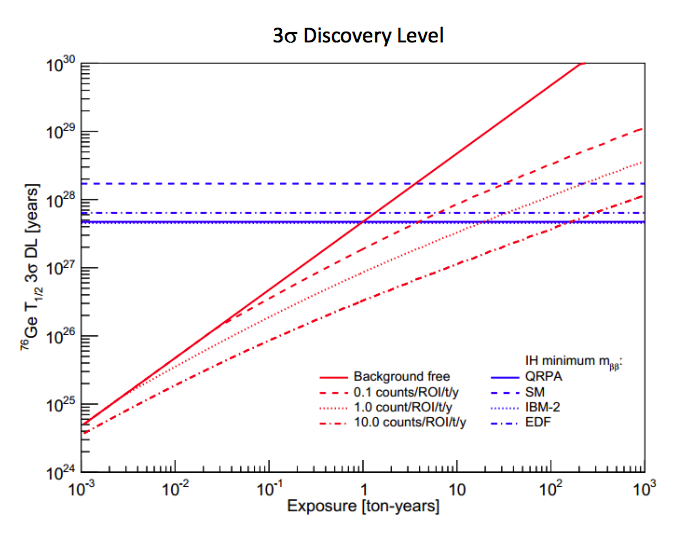
\includegraphics[width = \textwidth]{/Users/jgruszko/Documents/Thesis/Plots/Ch1/IH_Discovery.png}
\caption[The background requirements and exposure needed for $3\sigma$ discovery-level observation of $0\nu\beta\beta$ decay in the IH]{The background requirements and exposure needed for $3\sigma$ discovery-level observation of $0\nu\beta\beta$ decay, assuming the inverted hierarchy. The various red lines indicate the increase in sensitivity with increasing exposure for different background levels, and the blue lines indicate the bottom of the inverted hierarchy band in Fig.~\ref{fig:0nBBrate} under various nuclear matrix element calculation approaches. Plot courtesy of Jason Detwiler.}
\label{IH_Discovery}
\end{figure}

\section{The \MJ\ \DEM}\label{sec:MJD}
\subsection{The \DEM\ Apparatus}
The \MJ~\MJDemo, the $0\nu\beta\beta$ decay search that is the focus of much of this thesis, is an experiment made up of 44.8\,kg of PPC detectors. 29.7\,kg of this mass is enriched to 88\% \iso{76}{Ge}, and 15.1\,kg is in natural-abundance detectors. In addition to making a measurement of the \nonubb\ half-life comparable to that of other currently-operating experiments, its main experimental goals are:
\begin{itemize}
\item to demonstrate backgrounds low enough to justify construction of a tonne-scale experiment
\item to establish the feasibility of and techniques needed to construct and field modular arrays of Ge detectors
\item to search for additional physics beyond the Standard Model
\end{itemize}
The \DEM\ established a background goal of 3\,\cpRty\, assuming a 4\,keV ROI at the \nonubb\ Q-value. Accounting for self-shielding effects, this rate scales to 1\,\cpRty in a tonne-scale experiment, the maximum allowable background needed to fully explore the IH region with such an experiment. 

The \MJDemo~uses a staged, modular approach to construction (as seen in Fig.~\ref{fig:MJ_modular}), making its techniques naturally scalable to a tonne-scale experiment. All of the detectors in the \DEM are \ppc\ HPGe detectors, produced by ORTEC and Canberra. The detectors themselves are discussed in Ch~\ref{ch:HPGe_det}. Each of the 58 detectors is placed in a low-mass copper mount that holds the detector and a low-mass front-end (LMFE) board that provides the first stage of signal amplification. The mount provides contact to the detector for thermal cooling, high-voltage biasing, and signal readout. These detector mounts are stacked into ``strings" of three to five detectors, and each string is suspended from the cold-plate of a copper cryostat. Seven strings are housed in each of the two \MJ\ cryostats. Each cryostat has its own cooling and vacuum system; the cryostat together with its dedicated systems is called a ``module." 

\begin{figure}[t]
\centering
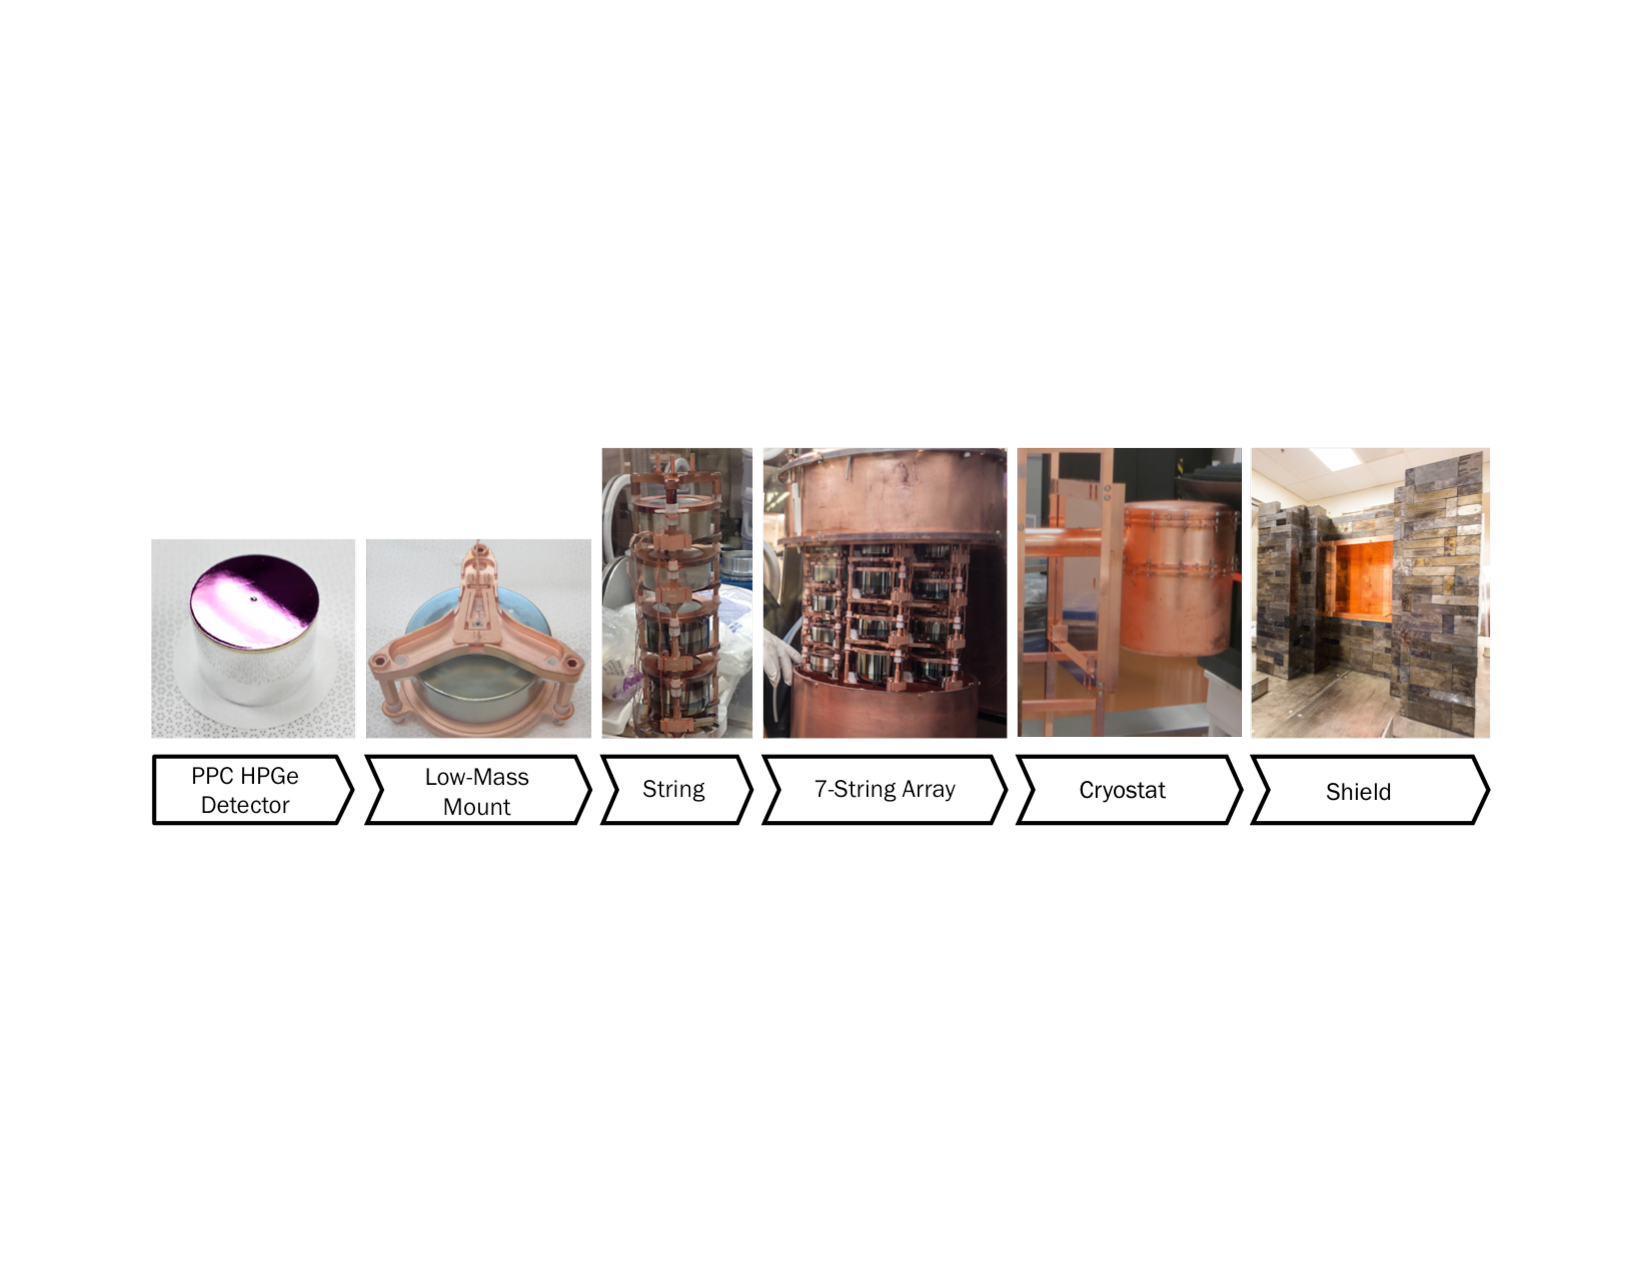
\includegraphics[width = \textwidth]{/Users/jgruszko/Documents/Thesis/Images/Ch1/MJD_design.pdf}
\caption[The modular elements of the \DEM\ design]{The \MJ\ \DEM\ uses a modular design approach. The \ppc\ detector shown is similar, though not identical, to those used in the \DEM. Photos by James Loach and Matt Kapust.}
\label{fig:MJ_modular}
\end{figure}

The two cryostats are inserted in a compact Cu and Pb shield and surrounded by a nitrogen-purged radon exclusion enclosure. Plastic scintillator veto panels surround the shield, detecting through-going cosmic muons, and and the modules are enclosed in high density polyethylene (HDPE) shielding to limit neutron backgrounds. The inner layers of the poly shielding are made of borated HDPE to provide further neutron capture. See Fig.~\ref{MJD_shield}. The \DEM\ is housed at the Davis Campus, at the 4850' level of the Sanford Underground Research Facility (SURF) \cite{MJD2014}. 

\begin{figure}[t]
\centering
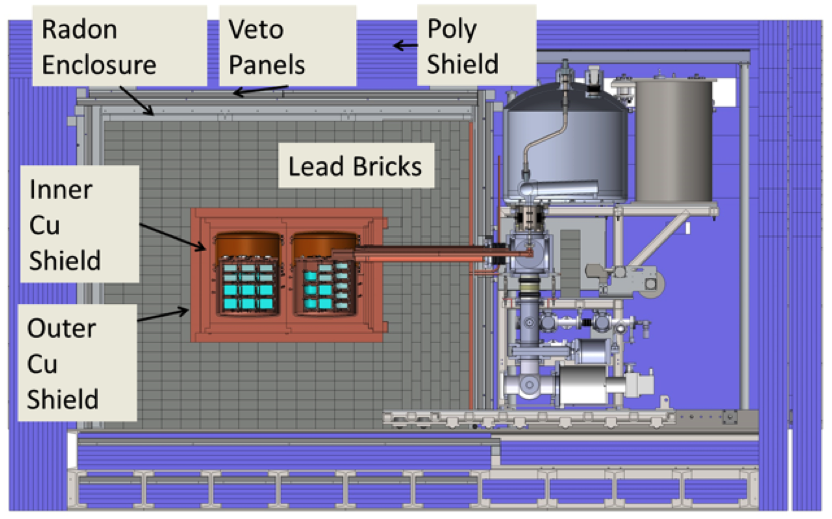
\includegraphics[height = 3in]{/Users/jgruszko/Documents/Thesis/Images/Ch1/MJD_shield.png}
\caption[A diagram of the \DEM\ shielding configuration]{A diagram of the \DEM\ showing the placement of the two cryostats, one of the two modules, the veto panels, and the shielding structure. The inner copper shield is made from underground electroformed copper, with the outer copper shield made from OFHC commercial copper. Diagram taken from \cite{MJD2014}.}
\label{fig:MJ_modular}
\end{figure}

The \DEM\ relies on ultra-low-background material selection and construction for its background reduction approach, with passive shielding to limit radioactive background events from the surrounding environment. The \DEM's main innovations in this area are the use of ultra-clean underground electroformed copper and the development of extremely low-background and low-noise front-end electronics. 

Electroforming copper effectively removes impurities, limiting the U and Th chain contamination of the material. By performing the electroforming and machining of the parts underground, the material's exposure to cosmic rays is also minimized. This prevents the formation of $^{60}$Co, another problematic long-lived isotope. The over-2000\,kg of copper made underground by the \MJ\ Collaboration has U and Th chain contamination levels of less than 0.1\,$\mu$Bq/kg each. This upper limit is better than the 0.3\,$\mu$Bq/kg goal set by the Collaboration \cite{MJD_assay}. This clean copper is used for almost all the parts found in the \DEM, from the mounts holding each detector to the cryostats and inner shielding layer. The use of this material, along with extensive clean material selection and assay programs, has led to an assay-based prediction of $< 3.5$ \cpRty\ of background events in the \DEM \cite{MJD_assay}. 

The LMFE developed for the \DEM\ has excellent noise performance \cite{MJD2014} while maintaining high radiopurity. This allows the LMFE to be mounted directly onto each detector, reducing capacitative noise in the system, and improving the \DEM's overall noise performance. In the search for \nonubb, there are two main benefits to this design. First of all, the extremely good resolution of the \DEM\ allows the use of a 3\,keV ROI \cite{EnergyUnidoc}, rather than the planned 4\,keV window. This reduces the background for \nonubb\ detection by 75\% for an equivalent contamination level in the experiment. Second of all, the fast rise-times and low noise of the LMFE and other developed electronics allow for good performance of multi-site event discrimination, described in Ch.~\ref{ch:HPGe_det}. 

The electronics design and low backgrounds of the \DEM, even at low energies, also allow the \MJ\ Collaboration to pursue additional BSM physics observations. In the search for low-mass WIMP dark matter candidates, solar axion scattering off of electrons, and a slew of other proposed new physics, the \DEM\ has shown sensitivity comparable to that of many dedicated experiments \cite{MJD_WIMP2017}. The \DEM's sensitivity to these processes will continue to increase as its exposure increases and as the analysis techniques used for near-threshold events are improved. 

\subsection{Construction of the \DEM}
To maintain material cleanliness, the \DEM\ was constructed in a class-1000 cleanroom. All parts internal to the shielding were placed under nitrogen purge immediately after surface cleaning to reduce Rn implantation. The detectors themselves were only exposed in nitrogen-purged spaces, and never to the air of the underground laboratory. The assembly of all elements internal to the cryostat, where the materials have line-of-site exposure to the detectors, was conducted in a class-10 continuously-purged glovebox. 

These efforts reduces the chance of the detectors being exposed to humidity, which increases their leakage current, degrading their resolution, and of all the materials being contaminated with U- and Th-containing dust, increasing backgrounds in the \DEM. The use of nitrogen-purged environments reduces the chance of contamination by  $^{226}$Rn or other isotopes in its decay chain, which pose problematic backgrounds for \nonubb\ detection. This source of background events is the focus of this thesis. 

To ensure that cleanliness standards were maintained and that the many detectors and strings were assembled in a repeatable and reliable way, extensive administrative controls were developed, as described in Appendix~\ref{app:QA}. These work-logging and quality control procedures allowed the \DEM\ to be successfully assembled by a rotating workforce, with many new researchers being trained in construction over the course of more than two years. Every part and procedure used in the experiment was also tracked in the Majorana Parts Tracking Database \cite{MJD_PTDB}, allowing the origin of any observed backgrounds to be investigated. 

\subsection{Operations}
The \DEM\ operations took a phased approach, allowing the start of low background data taking with Module 1 while Module 2 was being assembled. Module 1 began operations in May 2015, with Module 2 beginning data taking in May 2016. The \MJ\ \DEM's official transition to operations occurred in March 2017. 

The \DEM\ uses a statistical blinding approach; blinded data-taking has been ongoing since Dec. 31, 2015. The results discussed in Ch.~\ref{ch:MJ_rates} are from the open part of data sets 0 through 4, summarized in Table~\ref{tab:DS_summary}. 

Initial results from the \DEM, covering only the open portions of data sets 0 and 1, were reported at the XXVII International Conference on Neutrino Physics and Astrophysics in 2016 \cite{MJD_Nu16}. Using a background estimate window of 400\,keV surrounding $Q_\beta\beta$, these results reported a background index of $7.5^{+4.5}_{-3.4}$E-3\,\cpKkgy, corresponding to $23^{+13}_{-10}$\,\cpRty\ in a 3.1\,keV ROI.

Recent simulations by the \MJ\ Collaboration have shown that the 400\,keV background estimate window used to report these results includes several expected gamma peaks from background sources, and over-estimates the flat background rate in the \nonubb\ ROI. The change to a 350\,keV window that excludes these peaks, along with other improvements in analysis and the \DEM's increased exposure, result in a background index of $2.7^{+4.0}_{-1.7}$E-3\,\cpKkgy. This corresponds to $8.1^{+12.0}_{-5.1}$\,\cpRty\ in the now-appropriate 3.0\,keV ROI \cite{EnergyUnidoc}. These preliminary results, which are discussed in Ch.~\ref{ch:MJ_rates}, are consistent to within 1$\sigma$ with the \DEM\ assay- and simulation-based upper limit of the expected backgrounds. 
